
% --------------------------------
% 
% --------------------------------

\section{MCPS: Genotyping 150k Mexicans}

% -------------------------
% Methods ----
% -------------------------
\subsection{Methods}

% -------------------------
% Results ("Main findings")
% -------------------------
\subsection{Main findings}

\begin{frame}
    \frametitle{Main findings}
    \framesubtitle{Migration patterns}

    \begin{columns}
    
    % Column 1
    \begin{column}{0.5\textwidth}

       \begin{itemize}[noitemsep,topsep=0pt]
            \item There is a \textbf{\color{complement-1} lack} of migratory patterns
       \end{itemize} 
    \end{column}
    
    % Column 2
    \begin{column}{0.5\textwidth}
        \begin{figure}[htpb]
            \centering
            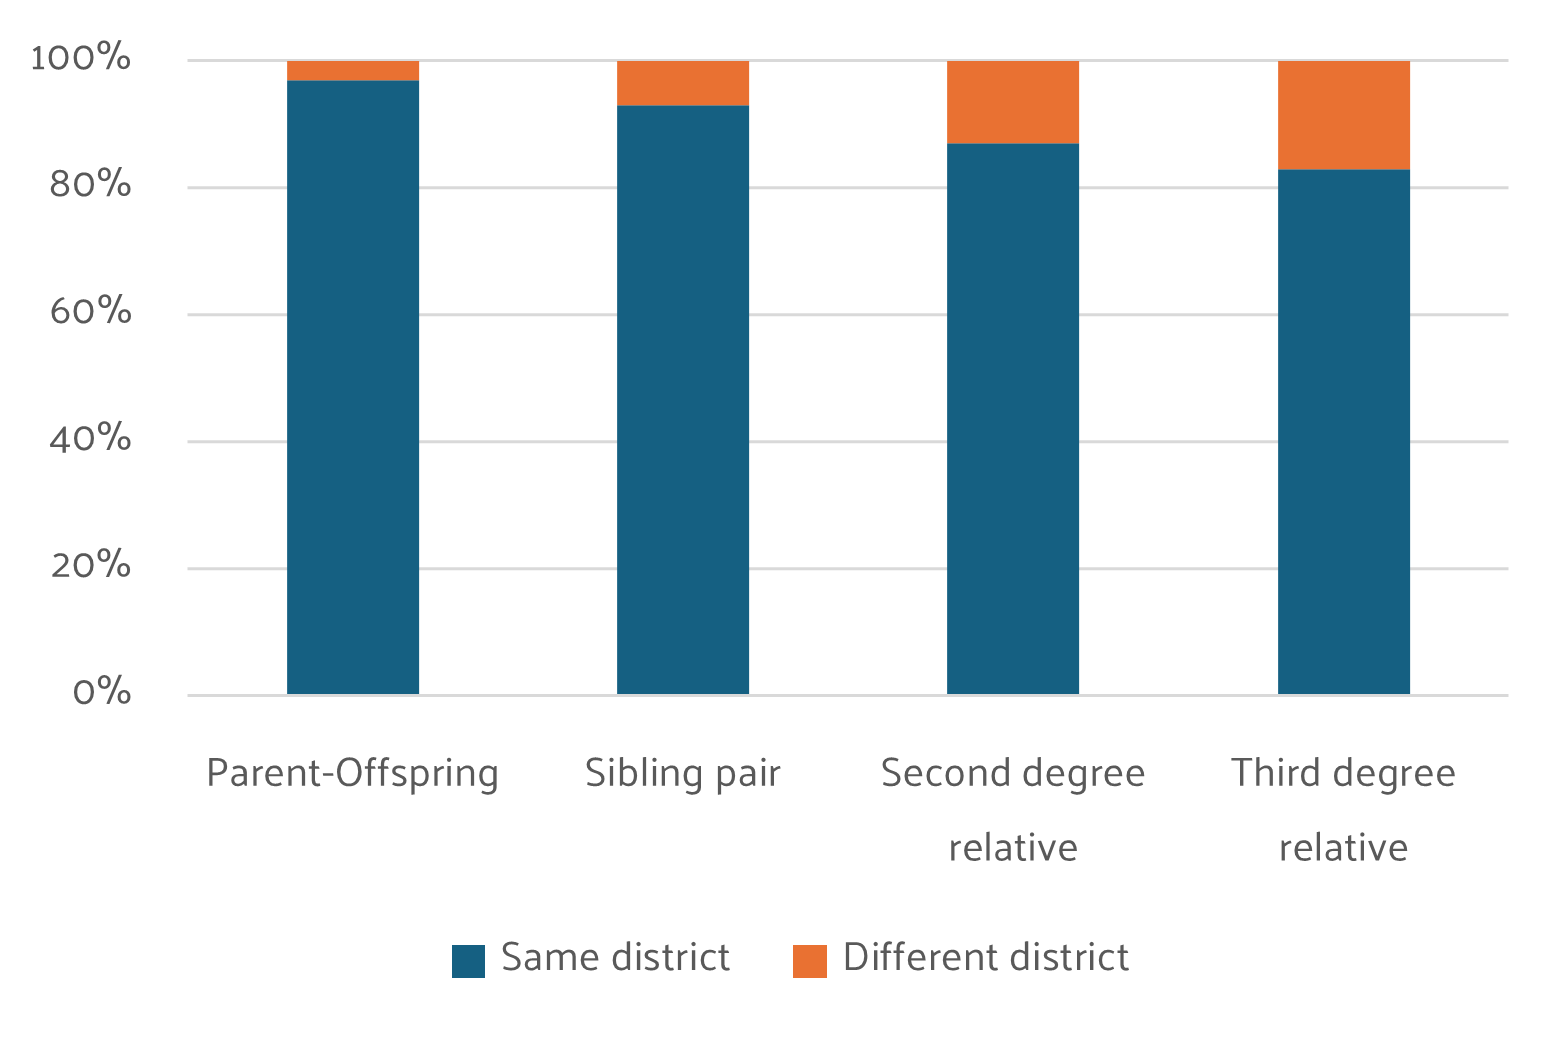
\includegraphics[width=0.95\textwidth]{ziyatdinov-2023/across-border.png}
            \caption{Proportion of relatives living across boundaries between Iztapalapa and Coyoacán \parencite{ziyatdinov2023}.}
            \label{fig:cross-border}
        \end{figure}
    \end{column}
    
    \end{columns}
    
\end{frame}

% Comparison of family networks
\begin{frame}
    \frametitle{Main findings}
    \framesubtitle{Dataset comparisons}

    % Please add the following required packages to your document preamble:
    % \usepackage{booktabs}
    % \usepackage[table,xcdraw]{xcolor}
    % Beamer presentation requires \usepackage{colortbl} instead of \usepackage[table,xcdraw]{xcolor}
    \begin{table}[]
    \caption{Comparison of family network sizes in MCPS, GHS and UKB datasets \parencite{ziyatdinov2023}.}
    \begin{tabular}{@{}cccc@{}}
    \toprule
    %\rowcolor{primary-color} 
    \textbf{}                                  & \textbf{MCPS   150k} & \textbf{GHS   145k} & \textbf{UKB   450k} \\ \midrule
    Parent-child relationships                 & 31,597 (33.1\%)      & 29,599 (31.1\%)     & 6,270 (2.3\%)       \\
    Full-sibling relationships                 & 29,482 (26.9\%)      & 18,540 (18.9\%)     & 22,657 (8.5\%)      \\
    2nd-degree relationships                   & 47,080 (31.2\%)      & 71,766 (42.4\%)     & 11,169 (4.2\%)      \\
    3rd-degree relationships                   & 120,180 (45.2\%)     & 129,782 (48.0\%)    & 66,847 (19.8\%)     \\
    Number of pedigrees                        & 22,766               & 19,770              & 24,560              \\
    Pedigrees with \textgreater{}2 individuals & 9,889                & 7,998               & 2590                \\
    Individuals with both parents (trios)      & 5,603                & 5,448               & 1,065               \\
    Pedigrees \textgreater{}2 generations      & 600                  & 2,299               & 0                   \\ \bottomrule
    \end{tabular}
    \label{tab:comparison-families}
    \end{table}
    
\end{frame}
